% $Author$ $Date$

%%%% for public version, toggle \draftfalse in setup2modes.tex
%    (that removes all comments, the blog)

% siminos/cgang/2modes.tex    this is master file:    pdflatex 2modes
%     then:    pdflatex def2modes; bibtex def2modes; pdflatex def2modes; pdflatex def2modes

\documentclass[aip,cha,reprint,
secnumarabic,
nofootinbib, tightenlines,
nobibnotes, showkeys, showpacs,
groupedaddress
%preprint,%
%author-year,%
%author-numerical,%
]{revtex4-1}

\newcommand{\version}{atlas ver. 0.2, Apr 30 2012}
% Predrag from atlas12      ver. 1.1, Apr 25 2012}

        \input setup2modes
        \input ../inputs/def
        \input def2modes

\begin{document}

\title[Low-dimensional cartography]
{Cartography of a 4-dimensional flow: A visual guide to sections and slices}

    \ifdraft
\author{Daniel Borrero-Echeverry}
\email{borrero@gatech.edu.}
\author{Keith M. Carroll}
\author{Bryce Robbins}
\author{Evangelos Siminos}
\author{Lei Zhang}
\date{\today}
\affiliation{
 School of Physics and School of Mathematics,
 Georgia Inst. of Technology,
 Atlanta, GA  30332, USA
}
    \else
\author{Bryce Robbins}
\author{Lei Zhang}
\date{1 May 2012}
\affiliation{
 School of Physics and School of Mathematics,
 Georgia Inst. of Technology,
 Atlanta, GA  30332, USA
 \\\\
 Georgia Tech PHYS 7224 spring 2012 course project
 \\
 \emph{Advisers:
 Predrag Cvitanovi\'{c},
 Daniel Borrero-Echeverry
 and
 Evangelos Siminos}
}
   \fi


    \begin{abstract}
Symmetry reduction by the method of slices [blah blah]
the role they play in organizing chaos.
    \end{abstract}

\pacs{02.20.-a, 05.45.-a, 05.45.Jn, 47.27.ed, 47.52.+j, 83.60.Wc}
\keywords{
symmetry reduction,
equivariant dynamics,
relative equilibria,
relative periodic orbits,
slices,
moving frames
}
\maketitle

    \begin{quotation}
Today, it is possible to  [blah blah].
    \end{quotation}

\section{Introduction}
\label{s:intro}

Over the last decade, new insights into the dynamics of  [blah blah]

Our goals here are ?-fold:
(i)  [blah blah].
(ii) [blah blah].

we shall illustrate the key ideas by a much
simpler example, the $\SOn{2}$-equivariant  [blah blah],

\section{Section}
\label{s:cut}


As an example consider the  [blah blah],

%%%%%%%%%%%%%%%%%%%%%%%%%%%%%%%%%%%%%%%%%%%%%%%%%%%%%%%%%%%%%%%%%%%%%
\begin{figure}
%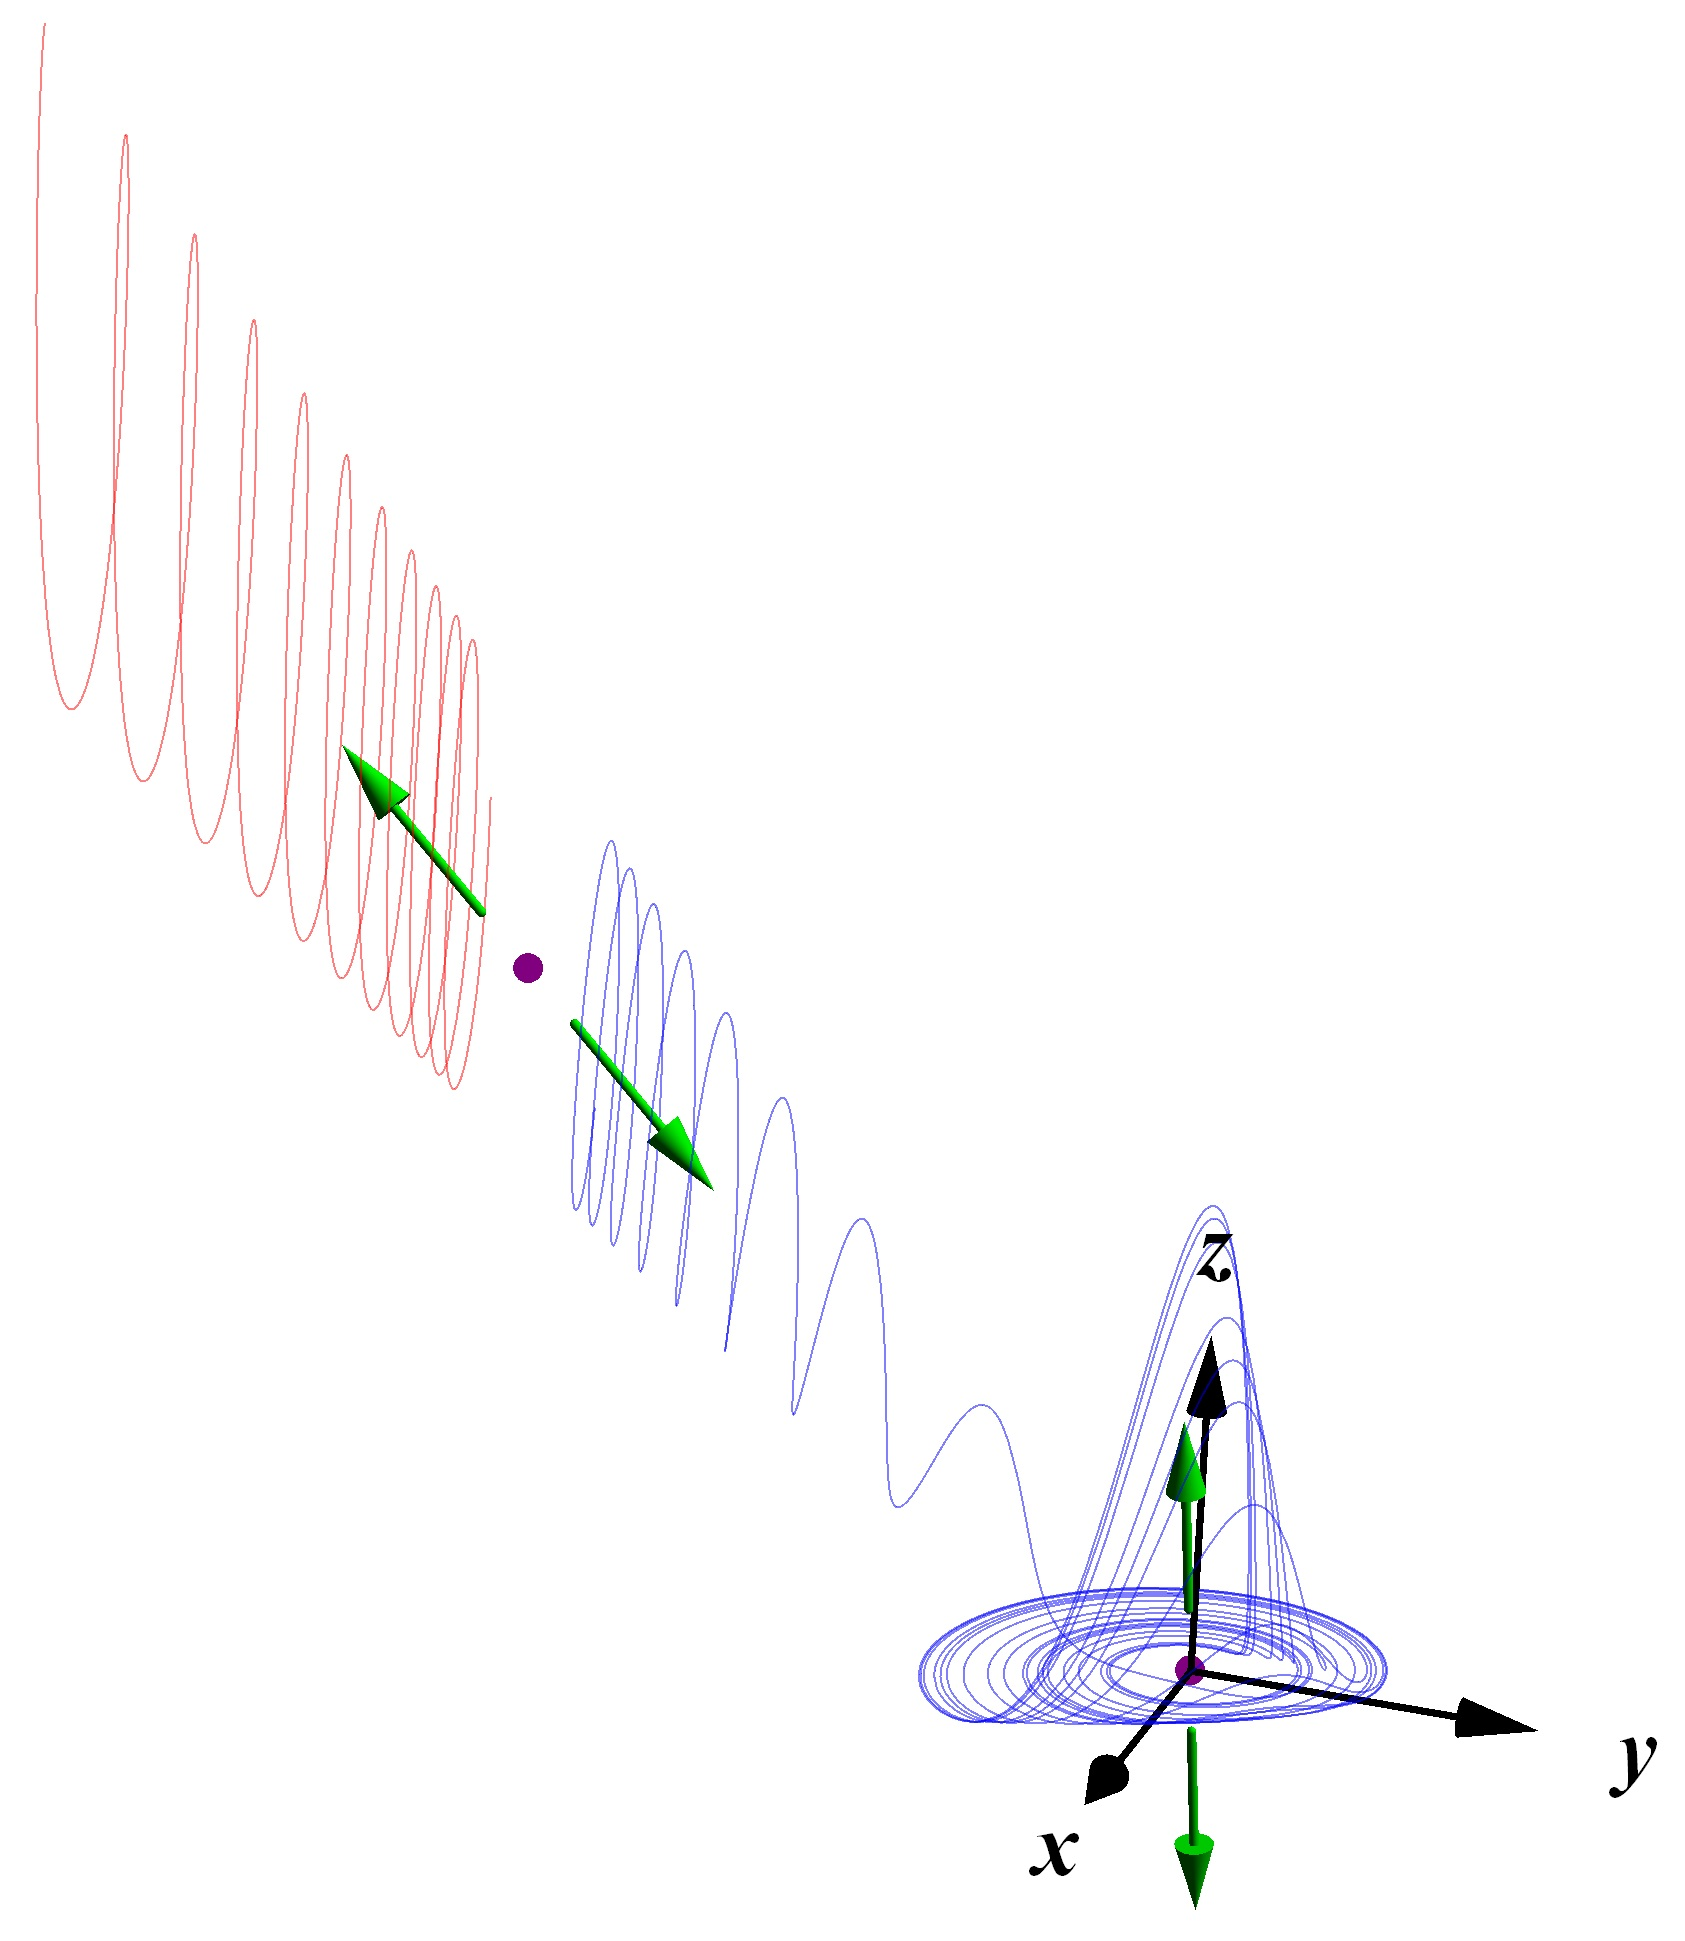
\includegraphics[width=0.28\textwidth]{RoessTrjs2}%{Rossler_Equilibria2}{RoessTrjs}%
 \begin{center}
 \setlength{\unitlength}{0.20\textwidth}
(a)
%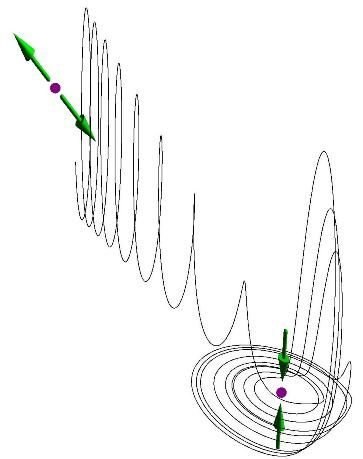
\includegraphics[width=\unitlength,clip=true]{RoessTrajLbld2}
(b)
%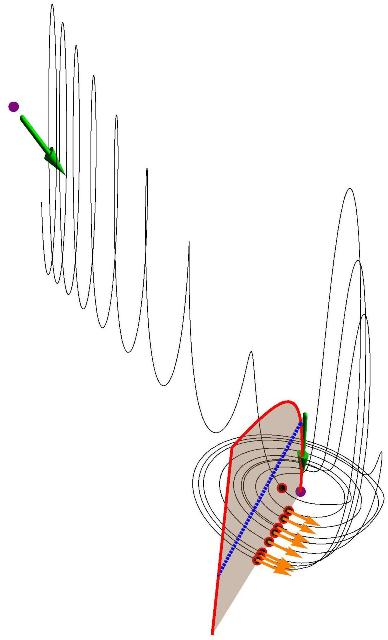
\includegraphics[width=\unitlength,clip=true]{RoessNeareqLbld2}
\\
(c)
%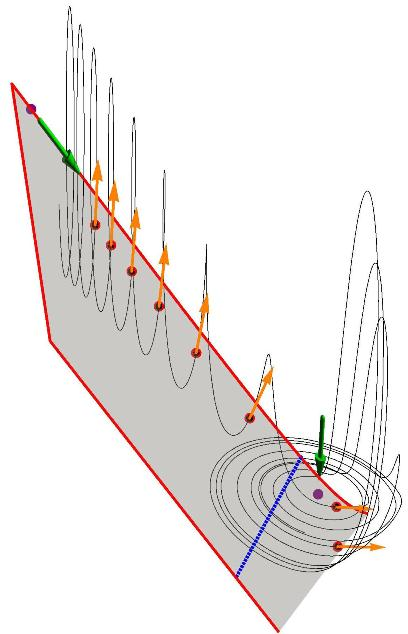
\includegraphics[width=\unitlength,clip=true]{RoessFareqLbld2}
(d)
%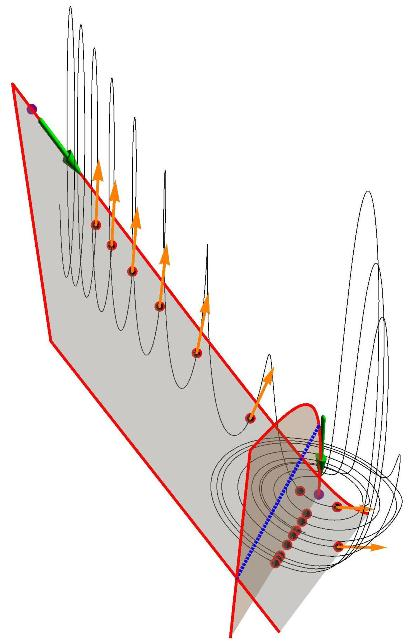
\includegraphics[width=\unitlength,clip=true]{RoessBotheqLbld2}
 \end{center}
    \caption{
2-chart atlas for \twoMode\ flow.
(a)
(b)
(c)
(d)
    }
\label{fig:2modeSects}
\end{figure}
%%%%%%%%%%%%%%%%%%%%%%%%%%%%%%%%%%%%%%%%%%%%%%%%%%%%%%%%%%%%%%%%%%%%%

 [blah blah]

\section{Dynamics and symmetry}
\label{s:symm}

\subsection{\twoMode\ $\SOn{2}$-equivariant flow}
\label{s:twoMode}

% \item[2012-04-28 Predrag]
Consider a system constructed from two Fourier modes
$m=(1,2)$,\rf{Dang86,AGHO288,PoKno05}, a representation of the symmetry
group $\SOn{2}$ defined by rotation
\beq
(z_1,z_2) \rightarrow   (e^{i {\gSpace}}z_1,e^{i 2{\gSpace}} z_2)
\,.
\ee{Dang86(1.1)aa}
$\SOn{2}$ invariant polynomials are
\bea
u &=& {z}_1 \overline{z}_1
    \,,\quad
v = {z}_2 \overline{z}_2
    \continue
w &=& z_1^2 \overline{z}_2 + \overline{z}_1^2 {z}_2
    \,,\quad
q = (z_1^2 \overline{z}_2 - \overline{z}_1^2 {z}_2)/\ii
\,,
\label{Dang86(1.2)PK}
\eea
The polynomials $\{u,v,w,q\}$ are
linearly independent, but related through one syzygy,
%2012-04-29 Double checked, added missing factors of 2 for w and q terms
%2012-04-29 Predrag: thanks!
\beq
w^2+q^2 - 4\,u^2v =0
  \,,
\label{eq:syzPK}
\eeq
confining the dynamics to a 3-dim\-ens\-ion\-al $\pS/\SOn{2}$ \reducedsp\
manifold, a
symmetry-invariant repre\-sent\-ati\-on of the 4-dim\-ens\-ion\-al
\SOn{2} equivariant dynamics.
The dynamical equations for $\{u,v,w,q\}$ follow from the chain rule
\( %beq
 \dot{ u}_i= ({\partial u_i}/{\partial x_j}) \, \dot{x}_j
 \,,
\) %ee{HilbChainRl}
upon substitution
$\{{z}_1\,,\overline{z}_1\,, {z}_2\,,\overline{z}_2 \}$ $\to$
$\{u,v,w,q\}$. This yields
\bea
  \dot{u} &=& \overline{z}_1 \dot{z}_1 + {z}_1 \dot{\overline{z}}_1 %Double checked DB 04-29-2012
\,,\qquad
  \dot{v} = \overline{z}_2 \dot{z}_2 + {z}_2 \dot{\overline{z}}_2 %Double checked DB 04-29-2012
\continue
  \dot{w} &=& 2 \,\overline{z}_2 {z}_1 \dot{z}_1 %Double checked DB 04-29-2012
           + 2\,{z}_2 \overline{z}_1 \dot{\overline{z}}_1
           + {z}_1^2 \dot{\overline{z}}_2
           + \overline{z}_1^2 \dot{z}_2
\continue
  \dot{q} &=&  (2\,\overline{z}_2 {z}_1 \dot{z}_1 %Double checked DB 04-29-2012
           - 2\,{z}_2 \overline{z}_1 \dot{\overline{z}}_1
           + {z}_1^2 \dot{\overline{z}}_2
           - \overline{z}_1^2 \dot{z}_2
           )/\ii
\label{PKinvEqs}
\eea

Dangelmayr,\rf{Dang86} Armbruster, Guckenheimer and Holmes,\rf{AGHO288}
Jones and Proctor,\rf{JoPro87} and Porter and Knobloch\rf{PoKno05} (see
Golubitsky \etal\rf{golubII}, Sect. XX.1) have investigated bifurcations
in 1:2 resonance ODE normal form models to third order in the amplitudes.
We shall study here a model of that type
that we shall refer to as the {\twoMode} system:
\begin{subequations}\label{eq:DangSO2}
\begin{align}
  \dot{z}_1 &= \mu_1\,z_1+a_1\,z_1|z_1|^2+b_1\,z_1|z_2|^2+c_1\,\overline{z}_1\,z_2\,\\
  \dot{z}_2 &= (\mu_2-\ii\, e_2)\,{z_2}+a_2\,z_2|z_1|^2+b_2\,z_2|z_2|^2+c_2\,z_1^2
\,,
\end{align}
\end{subequations}
with $z_1,\,z_2$  complex, and real valued  parameters. For parameters
far from bifurcation values the model has no physical motivation; in
particular, the parameter $(\mu_2-\ii\, e_2)$ is one of the many ways in
which $\On{2}$ symmetry of the Dangelmayr,\rf{Dang86} normal form system
can be broken to $\SOn{2}$ symmetry. We use the model to compare and
illustrate different symmetry reduction methods, in the dimensionally
lowest possible setting: a \statesp\ of dimension $d=4$, with the
$\SOn{2}$-reduced dynamics taking place in 3 dimensions, the lowest
possible if the dynamics is to be chaotic. Substituting the
$\SOn{2}$-equivariant system \refeq{eq:DangSO2} into \refeq{PKinvEqs} we
obtain a set of 4 invariant equations,
    \PC{2012-04-27 to Lei and all, please recheck! $e_2$ terms differ
    from Lei. DB 04-29: Double checked using computer algebra. Found a
    couple of discrepancies. Fixed them in red.}
\bea% Triple checked ES 04-30-2012
  \dot{u} &=& 2\,\mu_1\,u+2\,a_1\,u^2+2\,b_1\,u\,v+c_1\,w %Double checked DB 04-29-2012
\continue
  \dot{v} &=& 2\,\mu_2\,v+2\,a_2\,u\,v+2\,b_2\,v^2+c_2\,w %Double checked DB 04-29-2012
\continue
  \dot{w} &=& (2\,\mu_1+\mu_2)\,w+(2a_1+a_2)\,u\,w+(2b_1+b_2)\,v\,w %Double checked DB 04-29-2012 corrected coefficients for uv and u^2 terms
\ceq
             +\, \DBedit{4}c_1\,u\,v + \DBedit{2}c_2\,u^2 - e_2\,q
\label{PKinvEqs1}\\
  \dot{q} &=& (2\mu_1+\mu_2)\,q+(2a_1+a_2)\,u\,q+(2b_1+b_2)\,v\,q
             +e_2\,w %Double checked DB 04-29-2012
\nnu
\eea
One can now either investigate the dynamics in this invariant basis or
plot the `image'\rf{GL-Gil07b} of solutions computed in the equivariant
basis \refeq{eq:DangSO2} in terms of invariant polynomials
\refeq{Dang86(1.2)PK}.

In polar coordinates $ {z}_1 = |u|^{1/2} e^{\ii\theta_1}$, $ {z}_2 =
|v|^{1/2} e^{\ii\theta_2}$ the  $w, q$ invariants take form
\bea
w &=& 2\,\Re(z_1^2 \overline{z}_2) = 2\,u |v|^{1/2} \cos \psi %Double checked DB 04-29-2012
\continue
q &=& 2\,\Im(z_1^2 \overline{z}_2) = 2\,u |v|^{1/2} \sin \psi %Double checked DB 04-29-2012
\,,
\label{Dang86(1.2)polar}
\eea
where $\psi = 2 \theta_1 - \theta_2$.


%%%%%%%%%%%%%%%%%%%%%%%%%%%%%%%%%%%%%%%%%%%%%%%%%%%%%%%%%%%%%%%%%%%%%%%%%%%%%%%%%%%%%%%%%%%%%%%%%%
\subsection{To do}
\label{s:ToDo}

\begin{itemize}
	\item[10.?] The \twoMode\ system:
		\begin{itemize}
			\item(a) Show that the complex \twoMode\ system \refeq{eq:DangSO2}
			 may be rewritten as a 4-dimensional first order ODE system			
			\bea
				\dot{x}_1 &=& a_1 x_1^3 + b_1 x_1 y_1^2 + c_1 x_1 y_1 + a_1 x_1 x_2^2 + b_1 x_1 y_2^2 + \mu_1 x_1 + c_1 x_2 y_2
				\continue
				\dot{y}_1 &=& a_1 x_1^2 x_2 + c_1 x_1 y_2 + b_1 y_1^2 x_2 - c_1 y_1 x_2 + a_1 x_2^3 + b_1 x_2 y_2^2 + \mu_1 x_2
				\continue
				\dot{x}_2 &=& a_2 x_1^2 y_1 + c_2 x_1^2 + b_2 y_1^3 + a_2 y_1 x_2^2 + b_2 y_1 y_2^2 + \mu_2 y_1 - c_2 x_2^2 + e_2 y_2
				\continue
				\dot{y}_2 &=& a_2 x_1^2 y_2 + 2 c_2 x_1 x_2 + b_2 y_1^2 y_2 - e_2 y_1 + a_2 x_2^2 y_2 + b_2 y_2^3 + \mu_2 y_2
			\eea
						by substituting $z_1 = x_1 + i x_2$ and $z_2 = y_1 + i y_2$.
			
			\item(b) Now, show that the stability matrix ({\color{red}insert DasBuch eq. ref here, originally eq. 4.3}) A for this 				system is given by

\beq
A  \, =
\left( \begin{array}{cccc}
         3 a_1 x_1^2 + b_1 y_1^2 + c_1 y_1 + a_1 x_2^2 + b_1 y_2^2 + \mu_1 &  c_1 y_2 + 2 a_1 x_1 x_2 & c_1 x_1 + 2 b_1 x_1 y_1 & c_1 x_2 + 2 b_1 x_1 y_2 \\
        c_1 y_2 + 2 a_1 x_1 x_2  & a_1 x_1^2 + b_1 y_1^2 - c_1 y_1 + 3 a_1 x_2^2 + b_1 y_2^2 + \mu_1 & 2 b_1 y_1 x_2 - c_1 x_2 & c_1 x_1 + 2 b_1 x_2 y_2 \\
          2 c_2 x_1 + 2 a_2 x_1 y_1 & 2 a_2 y_1 x_2 - 2 c_2 x_2  & a_2 x_1^2 + 3 b_2 y_1^2 + a_2 x_2^2 + b_2 y_2^2 + \mu_2 & e_2 + 2 b_2 y_1 y_2\\
          2 c_2 x_2 + 2 a_2 x_1 y_2 & 2 c_2 x_1 + 2 a_2 x_2 y_2 & 2 b_2 y_1 y_2 - e_2 & a_2 x_1^2 + b_2 y_1^2 + a_2 x_2^2 + 3 b_2 y_2^2 + \mu_2
      \end{array} \right)
\,.
\ee{2modeStabMatrix}

\item(c) Now show that the \twoMode\ system is equivariant under infinitesimal SO(2) rotations
({\color{red}insert DasBuch eq ref here, originally 10.18}) by substituting the Lie algebra generator
    \beq
\Lg  \, =
\left( \begin{array}{cccc}
         0 & 1 & 0 & 0 \\
        -1 & 0 & 0 & 0 \\
         0 & 0 & 0 & 2\\
         0 & 0 & -2 & 0
      \end{array} \right)
\ee{LGTwoMode}
and A into into the equivariance condition ({\color{red}insert DasBuch
eq. ref. here, originally 10.24}).
\end{itemize}

  \item[10.10] $\SOn{2}$ equivariance of the {\twoMode} system
           for infinitesimal angles.
  \item[10.11] Visualizations of the 4-dimensional {\twoMode} system
  \item[10.1?] draw a group orbit for the {\twoMode} model
  \item[10.22] {\twoMode} system in polar coordinates (maybe skip).
  \item[10.23] The relative equilibria of the {\twoMode} system
  \item[10.24] Plotting the relative equilibria of
           the {\twoMode} system in invariant coordinates
  \item[10.25] Plotting the relative equilibria of
           the {\twoMode} system in Cartesian coordinates
  \item[10.2?] construct a 2-chart atlas for a {\twoMode} system
\end{itemize}


 [blah blah]

Mercader and Prat\rf{MePrKn01} might
be a candidate if we decide to go with $\On{2}$ symmetry since really the
Rayleigh-Benard problem has $\On{2} \times Z_2$ symmetry and they are really
talking about breaking the $Z_2$ part.

 [blah blah]


\begin{enumerate}
  \item
        compute analytically the \stabmat\ \Mvar\ in polar coordinates
  \item
        Study eigenvalues, keep playing with parameters. We would like
        -preferably- no \reqv\ to be attracting limit cycle, and several of
        the \reqva\ to be complex-pair unstable, leading to chaos, to be
        visualized and sliced in Cartesian coordinates.
  \item
        If you find a nice chaotic attractors, others can join in
        constructing an atlas for it. We just need one and only one
        example with non-trivial \chartBord s and at least 2 charts.
\end{enumerate}

 [blah blah]

\begin{itemize}
  \item $\REQV{}{1} = (r_1,r_2,\psi)=(0.0516508, 1.26311,?)$ and
        $\REQV{}{2} = (0.467095,0.2146,?)$
  \item their plots in the Cartesian coordinates
  \item $\dot{\theta}$ to see how slow/fast are they. $\dot{\theta}$
        might be related to 4th eigenvalue, when you go back
        to Cartesian coordinates
  \item stability eigenvalues, eigenvectors of the \eqv\ $\EQV{0}$ at
        origin, at your parameter values - if it is stable, everything
        just might fall into it and die.
  \item plots of small perturbations of the above \eqv\ and \reqva\ in
        the Cartesian coordinates to see whether the dynamics looks
        chaotic
  \item $\REQV{}{1}$: 2 large positive eigenvalues looks scary - probably
        nothing re-visits this \reqv. A mildly unstable complex pair
        would have been sweeter. You get complex eigenvalue by Hopf-bifurcating off a
        stable orbit, typically.
  \item $\REQV{}{1}$: Does either unstable eigenvalue become a complex
        eigenvalue pair in Cartesian coordinates?
  \item $\REQV{}{2}$: contracting eigenvalues have very small imaginary
        part, so the presumably just rocket toward the \reqv, not much
        spiraling there. At least the unstable eigenvalue seems slow
        compared to all other eigenvalues.
  \item $\REQV{}{1}$: Does the unstable eigenvalue become a complex
        eigenvalue pair in Cartesian coordinates?
\end{itemize}

 [blah blah]

the connection
of the constants in \refeq{eq:2modesDangSO2} with $e_2=0$ to the constants in
equation (2.3) of \refref{Dang86} with $n=2$, $m=1$ is $\mu_1=\nu\epsilon\alpha$,
$a_1=-\nu\epsilon$, $b_1=-\nu\epsilon\rho$, $c_1=-\nu\mu$, $\mu_2=\epsilon\beta$,
$a_2=-\epsilon\kappa$, $b_2=-\epsilon\epsilon'$, $c_2=\mu\mu'$.


 [blah blah]



%%%%%%%%%%%%%%%%%%%%%%%%%%%%%%%%%%%%%%%%%%%%%%%%%
% 2011-09-09, 2012-03-30 Predrag: add BeThMovFr to
%            continuous.tex overheads, and ChaosBook
% replace A27movFrame*.* everywhere
\begin{figure}
  	\begin{center}
  	\setlength{\unitlength}{0.20\textwidth}
  (a)
  	\begin{picture}(1,1.07802818)%
    	\put(0,0){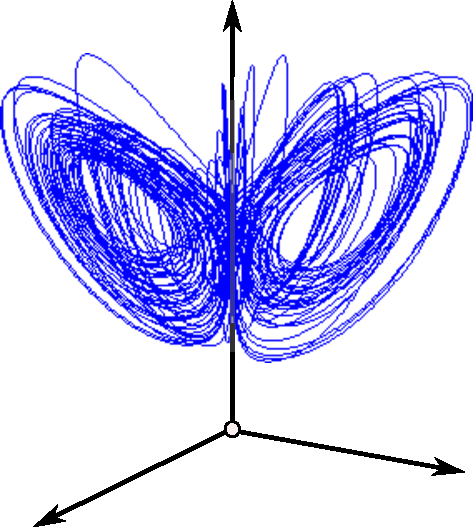
\includegraphics[width=\unitlength]{CLEattractor}}%
    	\put(0.55152995,1.0139628){\color[rgb]{0,0,0}\makebox(0,0)[lb]{\smash{$z$}}}%
    	\put(0.05573445,0.0739776){\color[rgb]{0,0,0}\makebox(0,0)[lb]{\smash{$x_1$}}}%
    	\put(0.90013492,0.16491708){\color[rgb]{0,0,0}\makebox(0,0)[lb]{\smash{$x_2$}}}%
  	\end{picture}%	
  (b)
  	\begin{picture}(1,1.06440474)%
    	\put(0,0){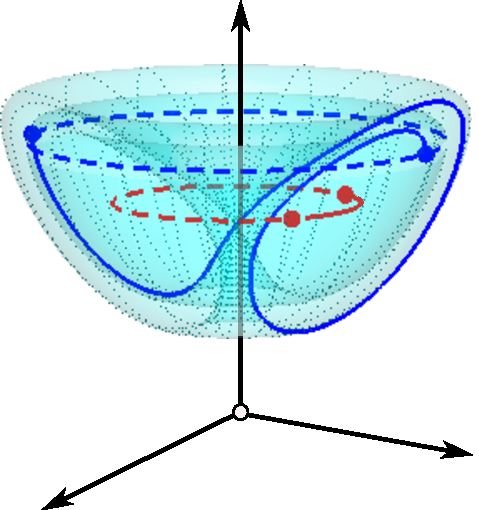
\includegraphics[width=\unitlength]{CLEWurst01}}%
   		\put(0.55961552,1.00214901){\color[rgb]{0,0,0}\makebox(0,0)[lb]{\smash{$z$}}}%
   		\put(0.07008555,0.07304272){\color[rgb]{0,0,0}\makebox(0,0)[lb]{\smash{$x_1$}}}%
    	\put(0.90381504,0.16283301){\color[rgb]{0,0,0}\makebox(0,0)[lb]{\smash{$x_2$}}}%
  	\end{picture}
\\
(c)   \begin{picture}(1,0.94310243)%
    \put(0,0){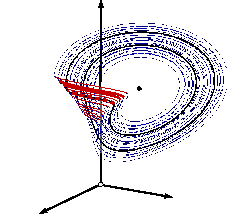
\includegraphics[width=\unitlength]{CLE1SliceSmall.pdf}}%
    \put(0.48564392,0.89244183){\color[rgb]{0,0,0}\makebox(0,0)[lb]{\smash{$z$}}}%
    \put(0.07181137,0.03185892){\color[rgb]{0,0,0}\makebox(0,0)[lb]{\smash{$y_2$}}}%
    \put(0.77031544,0.100183){\color[rgb]{0,0,0}\makebox(0,0)[lb]{\smash{$x_2$}}}%
  \end{picture}%
(d)   \begin{picture}(1,1.05662086)%
    \put(0,0){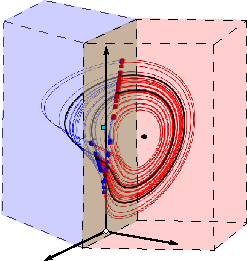
\includegraphics[width=\unitlength]{CLE2slicesmall.pdf}}%
    \put(0.47706962,0.83002768){\color[rgb]{0,0,0}\makebox(0,0)[lb]{\smash{$z$}}}%
    \put(0.08719004,0.02997825){\color[rgb]{0,0,0}\makebox(0,0)[lb]{\smash{$y_2$}}}%
    \put(0.73025395,0.09287946){\color[rgb]{0,0,0}\makebox(0,0)[lb]{\smash{$x_2$}}}%
  \end{picture}
    \end{center}
  \caption{
  \twoMode, $d=4 \to 3$~dimensional $\{x_1,x_2,z\}$ projections:
  (a)
  The strange attractor.
  (b)
 (c)
 In contrast
 to the 1\dmn\ \poincBord s of \reffig{fig:2modeSects}, here ...
 (d)
  }
\label{fig:2ModeAtlas}
\end{figure}
%%%%%%%%%%%%%%%%%%%%%%%%%%%%%%%%%%%%%%%%%%%%%%%%%%

 [blah blah]

 [blah blah]

\section{Chart}
\label{s:slice}

 [blah blah]

One can write the equations for the flow in the \reducedsp\
$\dot{\sspRed} = \velRed(\sspRed)$ (for details see, for example,
\refref{DasBuch}) as
\bea
\velRed(\sspRed) &=& \vel(\sspRed)
     \,-\, \dot{\gSpace}(\sspRed) \, \groupTan(\sspRed)
\label{2modesEqMotMFrame}\\
\dot{\gSpace}(\sspRed) &=& \braket{\vel(\sspRed)}{\sliceTan{}}
                       /\braket{\groupTan(\sspRed)}{\sliceTan{}}
\,
\label{2modesreconstrEq}
\eea
which confines the motion to the \slice\ hyperplane. Thus, the dynamical
system $\{\pS,\map^t\}$ with continuous symmetry \Group\ is replaced by
the {\reducedsp} dynamics $\{\pSRed,\mapRed^t\}$: The velocity in the
full \statesp\ $\vel$ is the sum of $\velRed$, the velocity component in
the \slice\ hyperplane, and $\dot{\gSpace}\,\groupTan$, the velocity
component along the group tangent space. The integral of the {\em
reconstruction equation} for $\dot{\gSpace}$ keeps track of the group
shift in the full \statesp.


 [blah blah]

\section{Charting the \slice}
\label{s:chart}

Let us summarize the voyage so far:

 [blah blah]


How the charts are put together is best told as a graphic tale, in the 5
frames of Figs.  [blah blah]



\section{Conclusions}
\label{s:concl}

 [blah blah]

\begin{acknowledgments}
This report addresses the questions asked in the  2012 Chaos course
[blah blah].
We are indebted to
 [blah blah]
and
 [blah blah]
for inspiring discussions.
\end{acknowledgments}


\bibliography{../bibtex/siminos}


\ifdraft
    \onecolumngrid

    \newpage
\input flotsam
    \newpage
    \section{{\twoMode} daily blog}
    \label{chap:2modes}
\input ../blog/2modes

\vfill
\begin{quote}
{\color{red} \large
May 1 2012,  11:30am - 2:20pm term projects due, Predrag's office
}
\end{quote}

\fi

\end{document}
